\documentclass{beamer}
\mode<presentation>
{
  \usetheme{Warsaw}
  \definecolor{mcgarnet}{rgb}{0.38, 0, 0.08}
  \definecolor{mcgray}{rgb}{0.6, 0.6, 0.6}
  \setbeamercolor{structure}{fg=mcgarnet,bg=mcgray}
  %\setbeamercovered{transparent}
}


\usepackage[english]{babel}
\usepackage[latin1]{inputenc}
\usepackage{times}
\usepackage[T1]{fontenc}
\usepackage{tikz}
\usepackage{graphicx}

\newcommand{\imagesource}[1]{{\centering\hfill\break\hbox{\scriptsize Image Source:\thinspace{\small\itshape #1}}\par}}

\title{Building Robust Programs}


\author{Robert Lowe\\}

\institute[Maryville College] % (optional, but mostly needed)
{
  Division of Mathematics and Computer Science\\
  Maryville College
}

\date[]{}
\subject{}

\pgfdeclareimage[height=0.5cm]{university-logo}{images/Maryville-College}
\logo{\pgfuseimage{university-logo}}



\AtBeginSection[]
{
  \begin{frame}<beamer>{Outline}
    \tableofcontents[currentsection]
  \end{frame}
}


\begin{document}

\begin{frame}
  \titlepage
\end{frame}

\begin{frame}{Outline}
  \tableofcontents
\end{frame}


% Structuring a talk is a difficult task and the following structure
% may not be suitable. Here are some rules that apply for this
% solution: 

% - Exactly two or three sections (other than the summary).
% - At *most* three subsections per section.
% - Talk about 30s to 2min per frame. So there should be between about
%   15 and 30 frames, all told.

% - A conference audience is likely to know very little of what you
%   are going to talk about. So *simplify*!
% - In a 20min talk, getting the main ideas across is hard
%   enough. Leave out details, even if it means being less precise than
%   you think necessary.
% - If you omit details that are vital to the proof/implementation,
%   just say so once. Everybody will be happy with that.

\section{The Problem}
\begin{frame}
    \frametitle{We Live in Uncertain Times}
    \begin{itemize}[<+->]
        \item There is no way to predict all environments and users of a program.
        \item Machines Break
        \item Disks Corrupt
        \item Internet Connections go Dark
        \item Users Remove USB Drives while you are reading them!
        \item Users have trouble distinguishing between numbers and words when you clearly ask for numbers.
    \end{itemize}
\end{frame}

\begin{frame}[fragile]
    \frametitle{Consider This Old Chestnut}
    \begin{verbatim}
#include <iostream>

using namespace std;

int getInt(string prompt)
{
    int x;
    
    cout << prompt;
    cin >> x;
    
    return x;
}
\end{verbatim}
\end{frame}

\begin{frame}[fragile]
    \frametitle{Consider This Old Chestnut}
    {\scriptsize
    \begin{verbatim}
int main()
{
    int x;
    int total=0;
    int count=0;
    
    do {
        x = getInt("Enter a number -1 to exit: ");
        if(x != -1) { 
            total+=x;
            count++;
        }
    } while(x != -1);
    
    cout << "Average: " << total/count << endl;
}
\end{verbatim}
}
\end{frame}

\begin{frame}[fragile]
    \frametitle{Everything is Fine With a Cooperative User!}
    \begin{verbatim}
Enter a number -1 to exit: 5
Enter a number -1 to exit: 5
Enter a number -1 to exit: 12
Enter a number -1 to exit: 7
Enter a number -1 to exit: -1
Average: 7
    \end{verbatim}
\end{frame}

\begin{frame}[fragile]
    \frametitle{However, One Smart Aleck Spoils the Game!}
    \begin{verbatim}
Enter a number -1 to exit: one
Enter a number -1 to exit: Enter a number -1 to 
exit: Enter a number -1 to exit: Enter a number 
-1 to exit: Enter a number -1 to exit: Enter a 
number -1 to exit: Enter a number -1 to exit: 
Enter a number -1 to exit: Enter a number -1 
to exit: Enter a number -1 to exit: Enter a 
number -1 to exit: Enter a number -1 to exit: 
Enter a number -1 to exit: 
    \end{verbatim}
\end{frame}

\begin{frame}
    \frametitle{We Need to Build Foolproof\footnotemark Programs!}
    
    \begin{itemize}[<+->]
        \item The solution to this problem is proper use of {\bf exceptions}.
        \item An exception is a deviation from the normal flow of a program.
        \item This works outside of the normal return scheme of functions.
        \item Even void functions can have exceptions!
        \item Before we look at exceptions, we need to understand some low level things about function calls.
    \end{itemize}
    
    \footnotetext[1]{Nothing is foolproof to a sufficiently talented fool. (Murphy's Law)}
\end{frame}

\section{An Overview of Stack Frames}
\begin{frame}
    \frametitle{Stacks}
    \begin{itemize}[<+->]
        \item A stack is a basic data structure.
        \item Stacks have two fundamental operations: push and pop.
        \item Pushing an item onto a stack puts it on top.
        \item Popping an item from a stack removes the top element.
        \item It's just like stacking up books or papers!
    \end{itemize}
\end{frame}
\begin{frame}
    \frametitle{The Big Idea}
    {\bf When you call a function...}
    \begin{enumerate}[<+->]
        \item Function parameters are pushed onto the call stack.
        \item The return address is pushed onto the call stack.
        \item Control is transferred to the function.
        \item The function pushes any local variables it may have onto the call stack.
    \end{enumerate}
    {\bf When a function returns...}
    \begin{enumerate}[<+->]
        \item A magic gnome is given your return value for safe keeping.
        \item All local variables are popped off the stack.
        \item The return address is popped off the stack, and control is
            transferred to that location.
        \item Parameters are all popped off the stack.
    \end{enumerate}
    
\end{frame}
\begin{frame}[b]
    \frametitle{An Example Call Stack}
    \begin{columns}
        \column[b]{0.5\textwidth}
        \begin{enumerate}
            \item[3]<4-|handout:3-> Function {\tt g} is called, It's frame is pushed on the stack
            \par\vspace{0.3in}
            \item[2]<3-|handout:2-> Function {\tt f} is called, It's frame is pushed on the stack.
            \par\vspace{0.3in}
            \item[1]<2-|handout:1-> {\tt main} Function is Called.  It's stack frame is pushed on the stack.
            \par\vspace{0.25in}
        \end{enumerate}
        \column[b]{0.5\textwidth}
            \begin{overlayarea}{\textwidth}{0.9\textheight} 
                \only<2|handout:1>{\vspace{1.82in}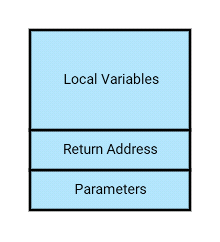
\includegraphics[width=1in,height=0.91in]{images/callStack1}}
                \only<3|handout:2>{\vspace{0.91in}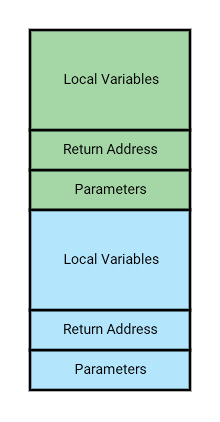
\includegraphics[width=1in,height=1.82in]{images/callStack2}}
                \only<4|handout:3>{\vspace{0in}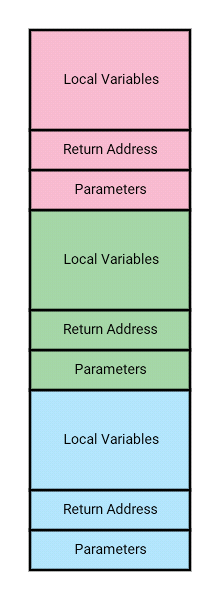
\includegraphics[width=1in,height=2.75in]{images/callStack3}}
            \end{overlayarea}
    \end{columns}
\end{frame}

\section{Exception Handling}
\begin{frame}
    \frametitle{Throwing Exceptions}
    \begin{itemize}[<+->]
        \item How can we report an exception?
        \item One way would be to use the return value of the function.
        \item This creates two problems!
        \begin{itemize}
            \item Void functions have no way to report errors.
            \item This removes one (or more) of the possible return values from a function.
        \end{itemize}
        \item C++ Provides a much better way, throwing exceptions!
        \item Any data type can be "thrown" from a function.
    \end{itemize}
\end{frame}

\begin{frame}[fragile]
    \frametitle{Error Checking in {\tt getInt}}
    {\small
    \begin{verbatim}
int getInt(string prompt)
{
    int x;
    
    cout << prompt;
    cin >> x;
    
    if(not cin) {
        throw invalid_argument("User input not valid");
    }
    
    return x;
}
\end{verbatim}
}
\end{frame}

\begin{frame}[fragile]
    \frametitle{Let's See our Smart Aleck Now!}
    \begin{verbatim}
Enter a number -1 to exit: one
terminate called after throwing an instance of 
'std::invalid_argument'
  what():  User input not valid
Aborted (core dumped)
    \end{verbatim}
\end{frame}

\begin{frame}
    \frametitle{A Note About Standard Streams}
    \begin{itemize}[<+->]
        \item Standard streams contain an overloaded operator which casts a stream to {\tt bool}
        \item When an error occurs in translation, this will cause the stream to return false when cast to bool.  Otherwise it returns true.
        \item The {\tt clear()} method clears the error flags of a stream.
    \end{itemize}
\end{frame}

\begin{frame}[b]
    \frametitle{Why Did the Program Terminate?}
    \begin{columns}
        \column[b]{0.5\textwidth}
        \begin{enumerate}
            \item[1]<2-|handout:1-> {\tt getInt} throws an exception.  This terminates the function.
            \par\vspace{0.3in}
            \item[2]<3-4|handout:2-4> {\tt main} does not catch the exception, so it is also terminated.
            \par\vspace{0.25in}
        \end{enumerate}
        \column[b]{0.5\textwidth}
            \begin{overlayarea}{\textwidth}{0.9\textheight} 
                \only<1-2|handout:1-2>{\vspace{0.91in}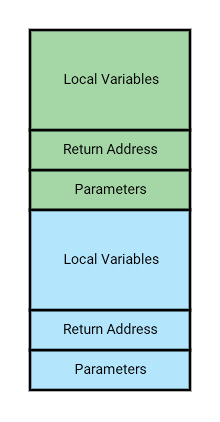
\includegraphics[width=1in,height=1.82in]{images/callStack2}}
                \only<3|handout:3-3>{\vspace{1.82in}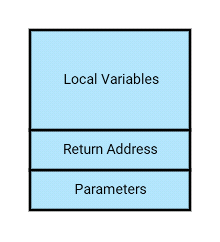
\includegraphics[width=1in,height=0.91in]{images/callStack1}}
            \end{overlayarea}
    \end{columns}
\end{frame}

\begin{frame}
    \frametitle{Catching an Exception}
    \begin{itemize}[<+->]
        \item C++ provides a {\tt try...catch} block for catching exceptions.
        \item If code within a try block throws an exception, it can be caught by a catch block.
        \item Exceptions are caught by type.
    \end{itemize}
\end{frame}

\begin{frame}[fragile]
    \frametitle{Modifying Main to Catch an Exception}
    {\small
    \begin{verbatim}
//same beginning
try {
  x = getInt("Enter a number -1 to exit: ");
} catch(const invalid_argument &ex) {
  cerr << "Invalid entry.  Please try again." << endl;
    
  //clear out the wayward input and reset flags
  cin.clear();
  cin.ignore(numeric_limits<streamsize>::max(), '\n');
    
  //try again
  continue;
}
// the rest remains unchanged
    \end{verbatim}
}
\end{frame}

\begin{frame}[fragile]
    \frametitle{Let's Give Our Friend One Last Go}
    \begin{verbatim}
Enter a number -1 to exit: one
Invalid entry.  Please try again.
Enter a number -1 to exit: one
Invalid entry.  Please try again.
Enter a number -1 to exit: one
Invalid entry.  Please try again.
Enter a number -1 to exit: 4
Enter a number -1 to exit: 5
Enter a number -1 to exit: 2
Enter a number -1 to exit: two
Invalid entry.  Please try again.
Enter a number -1 to exit: 3
Enter a number -1 to exit: -1
Average: 3
    \end{verbatim}
\end{frame}

\begin{frame}
    \frametitle{Best Practices When Using Exceptions}
    \begin{itemize}[<+->]
        \item If a chance for an exception exists, write code which will throw it!
        \item Where possible, use an existing exception object (see {\tt std::exception} for a list.)
        \item A try block can be followed by multiple catches.  If a block can throw multiple exceptions, catch all that you can handle.
        \item If you cannot handle an exception, don't catch it.  Let it pass further up the stack!
        \item Avoid writing catch-all blocks.  I'm not even going to show you how to do it.  You should only catch specific exceptions!
        \item Be careful of polymorphism!  Put more specific catches above more general catches.
    \end{itemize}
\end{frame}


\end{document}


